\documentclass{tufte-handout}

\usepackage{graphicx,amsmath}

\title{Probability Distributions}
\author{M. Henry Linder}
\date{}

\begin{document}
\maketitle

\section{Poisson Distribution}
The Poisson distribution is defined for $x = 0, 1, 2, \dots$

\begin{figure}
    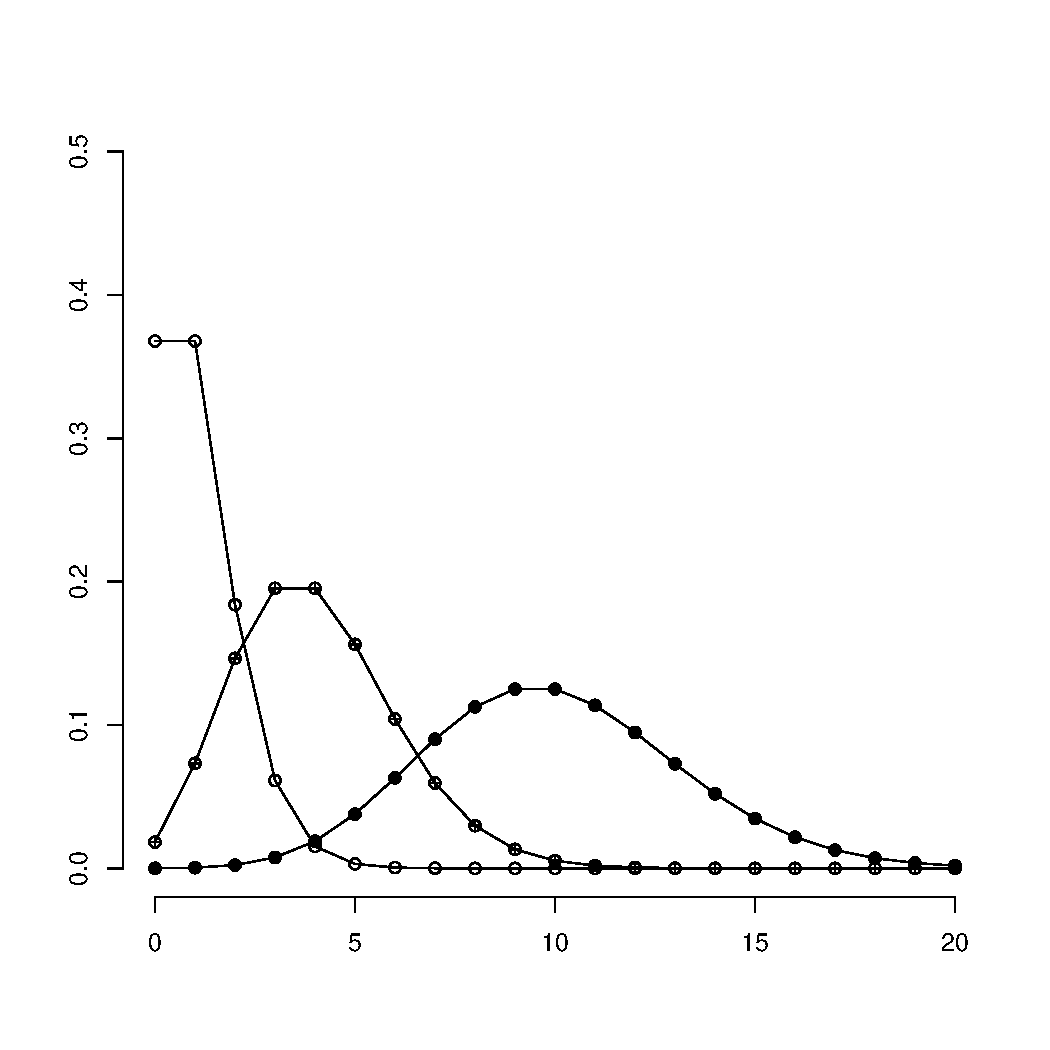
\includegraphics[width=\textwidth]{poisson_bw.pdf}
    \caption{Poisson Distribution for Various $\lambda$}
\end{figure}
\marginnote[-4.0in]{
    \begin{align*}
        & x = 0, 1, 2, \dots \\
        & 0 < \lambda < \infty \\
        & p(x) = \frac{e^{-\lambda}\lambda^x}{x!} \\
        & \mu = E[X] = \lambda \\
        & \sigma^2 = E[(x-\mu)^2] = \lambda \\
    \end{align*}
    }
\end{document}
